%% --------------------------------------------------------------
%%
%% I N T R O D U C T I O N
%%
%% --------------------------------------------------------------
\section{Introduction}



% =============================================================================================

\begin{frame}{}  %% ---------- Intro/motivation 
    \begin{tikzpicture}[overlay,remember picture]
        
        \uncover<1->{ % <-> |
            \node (t1) [anchor=center,scale=1,opacity=1] at ([shift={(-3.5cm,-0.5cm)}]current page.center){
                \parbox{0.6\textwidth}{
                    \begin{itemize}
                        \item One of the ways to understand the properties of matter at supernuclear densities 
                        is to study EM signatures of BNS, NSBH mergers and CCSNe. 
                        %
                        \item Non-thermal EM signatures: GRBs, kN afterglows, ... 
                        %
                        \item Origin: interaction between transrelativistic ejecta and ISM. 
                        %
                        \item Thus study of GRBs, kN probe the ejecta properties and by extension, the 
                        properties of the postmerger/post-SNe remnant. 
                        \item NR simulations + observations show 
                    \end{itemize}
            }};
            
        }
        \uncover<1-1>{ % <-> |
            \node (img1) [anchor=center,scale=1,opacity=1] at ([shift={(5.6cm,-0.8cm)}]current page.center){
                \parbox{0.5\textwidth}{
                    \includegraphics[height=7.0cm]{figures/Ascenzi20_EjectaEMPicture.pdf}
                    
                    %\small{\textbf{Artist depiction of ejecta$^\text{\citep{Ascenzi:2020xqi}}$}}
            }};
        }
    \end{tikzpicture}
\end{frame}


% =============================================================================================

\section{GRB afterglow}
\begin{frame}{}  %% ---------- Intro/motivation 
    \begin{tikzpicture}[overlay,remember picture]
        \uncover<1->{ % <-> |
            \node (t1) [anchor=center,scale=1,opacity=1] at ([shift={(-3.2cm,-0.5cm)}]current page.center){
                \parbox{0.65\textwidth}{
                    \textbf{Main Features}:
                    \begin{itemize}
                        \item Short \& Long
                        %
                        \item Three main stages: thermal/photosphere, prompt, \textbf{afterglow}
                         ( flares, shallow rise, rebrightening$(^*)$ )
                        %
                        \item Display plateus, flares, rebrightening($^*$)
                        %
                        \item Afterglow: synchrotron emission from (and forward shock). 
                        %
                    \end{itemize}
                    
                    \textbf{Key observables}:
                    \begin{itemize}
                        \item $F_{\nu;p}\propto E_{\rm iso} n_{\rm ISM}^{(p+1)/4}\theta_{\rm obs}^{-2p}\varepsilon_e^{p-1}\varepsilon_B^{(p+1)/4}D_{L}\nu^{(1-p)/2}$
                        \item $t_p\propto E_{\rm iso}^{1/3}n_{\rm ISM}^{-1/3}\theta_{\rm obs}^2$
                        \item Jet composition (Baryonic vs Poyniting flux)
                        \item Late-time engine activity 
                    \end{itemize}
            }};
            
        }
        \uncover<1-1>{ % <-> |
            \node (img1) [anchor=center,scale=1,opacity=1] at ([shift={(4.5cm,1.4cm)}]current page.center){
                \parbox{0.5\textwidth}{
                    \includegraphics[height=4.2cm]{figures/grb_xray_canonic.png}
                    
                    %\small{\textbf{Artist depiction of ejecta$^\text{\citep{Ascenzi:2020xqi}}$}}
            }};
        }
        \uncover<1-1>{ % <-> |
            \node (img1) [anchor=center,scale=1,opacity=1] at ([shift={(5.0cm,-2.4cm)}]current page.center){
                \parbox{0.5\textwidth}{
                    \includegraphics[height=3.8cm]{figures/Ghirlanda19_GRB170817A.pdf}
                    
            }};
        }
    \end{tikzpicture}
\end{frame}


% =============================================================================================
\section{kN afterglows}
\begin{frame}{}  %% ---------- Intro/motivation 
    \begin{tikzpicture}[overlay,remember picture]
        \uncover<1->{ % <-> |
            \node (t1) [anchor=center,scale=1,opacity=1] at ([shift={(-3.1cm,-0.5cm)}]current page.center){
                \parbox{0.68\textwidth}{
                    \textbf{Main Features}:
                    \begin{itemize}
                        \item Synchrotron emission from mildly relativistic ejecta
                        (similar to GRB afterglow and SNe remnants)
                        %
                        \item Expected in sGRBs but have not observed$(^*)$
                        %
                        \item Complex ejecta structure/geometry $\rightarrow$ non-trivial EM signature
                        %
                    \end{itemize}
                    
                    \textbf{Key Observables}: 
                    \begin{itemize}
                        \item $F_{\nu,p}\propto E n^{(p+1)/4}\beta^{(5p-7)/2}\varepsilon_e^{p-1}\varepsilon_B^{(p+1)/4}D_L^{-2}\nu^{(-p-1)/2}$
                        \item $t_{p}\propto E^{1/3} n^{-1/3} \beta^{-5/3}$
                        %
                        \item Timescale of years.
                        %
                        \item Trace the properties of the fastest ejecta
                        %
                    \end{itemize}
            }};
        }
        \uncover<1-1>{ % <-> |
            \node (img1) [anchor=center,scale=1,opacity=1] at ([shift={(5.2cm,-4.2cm)}]current page.center){
                \parbox{0.5\textwidth}{
                    \includegraphics[height=8.6cm]{figures/afterglow_example.png}
                
                %\small{\textbf{Artist depiction of ejecta$^\text{\citep{Ascenzi:2020xqi}}$}}
            }};
        }
    \end{tikzpicture}
\end{frame}


% =============================================================================================

\section{Geometry}
\begin{frame}{}  %% ---------- Intro/motivation 
    \begin{tikzpicture}[overlay,remember picture]
        \uncover<1->{ % <-> |
            \node (t1) [anchor=center,scale=1,opacity=1] at ([shift={(-3.5cm,-0.5cm)}]current page.center){
                \parbox{0.6\textwidth}{
                    \textbf{Goal: combine structured GRB and kilonova afterglows}. \\
                    \textbf{Key features}:
                    \begin{itemize}
                        \item lateral structure \& lateral spreading of GRB ejecta
                        \item lateral \& velocity structure of kilonova ejecta
                        \item GRB jet evacuates ISM in front of ejecta
                        \item thermal electrons contribute to synchrotron emission from kilonova ejecta
                    \end{itemize}
            }};
            
        }
        \uncover<1-1>{ % <-> |
            \node (img1) [anchor=center,scale=1,opacity=1] at ([shift={(4.5cm,-0.5cm)}]current page.center){
                \parbox{0.5\textwidth}{
                    \includegraphics[height=7.2cm]{figures/structure.png}
                    
            }};
        }
    \end{tikzpicture}
\end{frame}



% =============================================================================================




%\section{Phsyics}
\subsection{Spectral evolution of GRB170817A}
\begin{frame}{}  %% ---------- Intro/motivation 
    \begin{tikzpicture}[overlay,remember picture]
        \uncover<1->{ % <-> |
            \node (t1) [anchor=center,scale=1,opacity=1] at ([shift={(-3.5cm,1.7cm)}]current page.center){
                \parbox{0.6\textwidth}{
                    GRB170817 from [Hajela et al 2021]:
                    \begin{itemize}
                        %                        \item late-time cahnge in afterglow (not a jet)
                        \item Statistical fit indicates
                        \textit{harder radio-to-X-ray spectrum} (lower $p$)
                        \item Radio obs. $\rightarrow$ optically thin spectrum
                        \item Lower $p=2$ \textit{is expected} in non-relativistic shocks (but with lower $\varepsilon_e$ as well)
                    \end{itemize}
                    
            }};
        }
        \uncover<1-1>{ % <-> |
            \node (img1) [anchor=center,scale=1,opacity=1] at ([shift={(5.0cm,0.1cm)}]current page.center){
                \parbox{0.5\textwidth}{
                    \includegraphics[height=6.5cm]{figures/figure4_2021paper.pdf}
            }};
        }
        \uncover<1-1>{ % <-> |
            \node (img1) [anchor=center,scale=1,opacity=1] at ([shift={(-3.0cm,-2.cm)}]current page.center){
                \parbox{0.5\textwidth}{
                    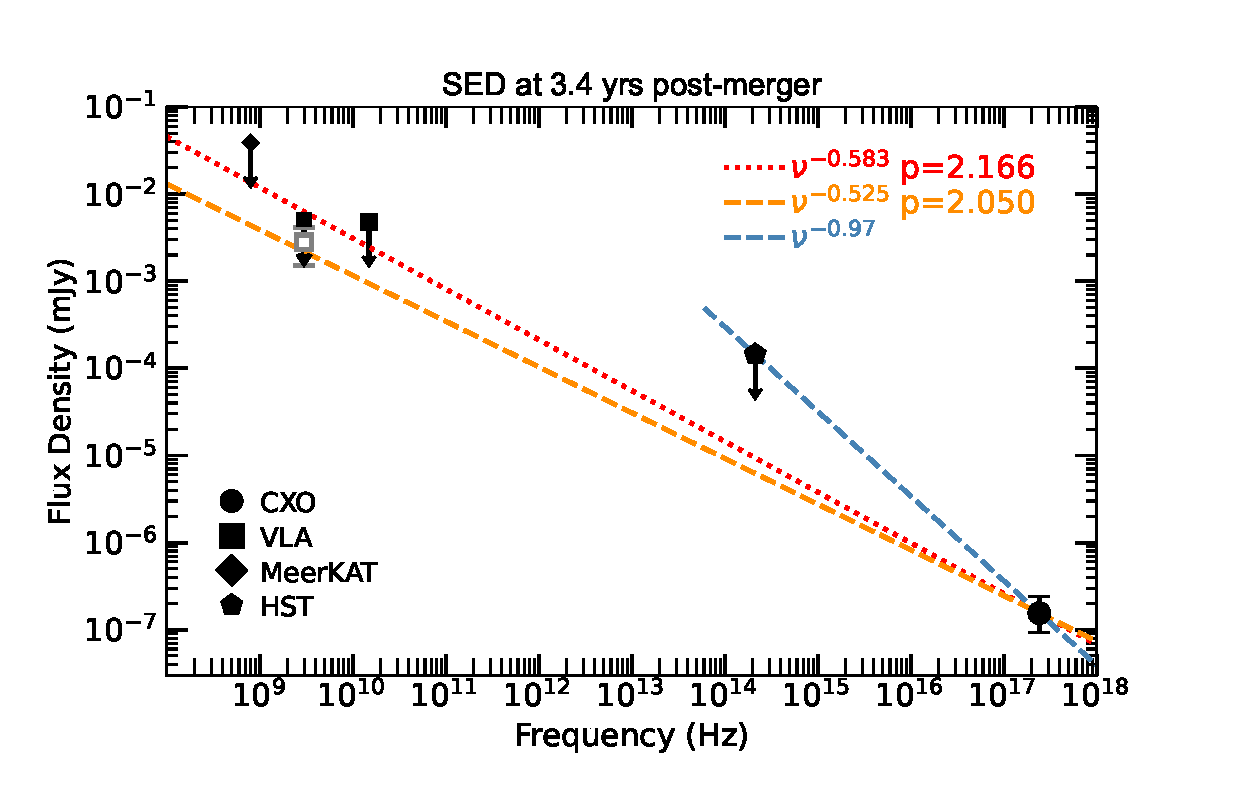
\includegraphics[height=4.5cm]{figures/SED1234days.eps}
            }};
        }
    \end{tikzpicture}
\end{frame}

